% RNA codons
% Author: Florian Hollandt

\documentclass{article}

%\usepackage{Florian}

\usepackage{tikz}

\setlength\oddsidemargin{0in}
%\setlength\evensidemargin{0in}


\begin{document}


\tiny

\pagestyle{empty}

\begin{center}
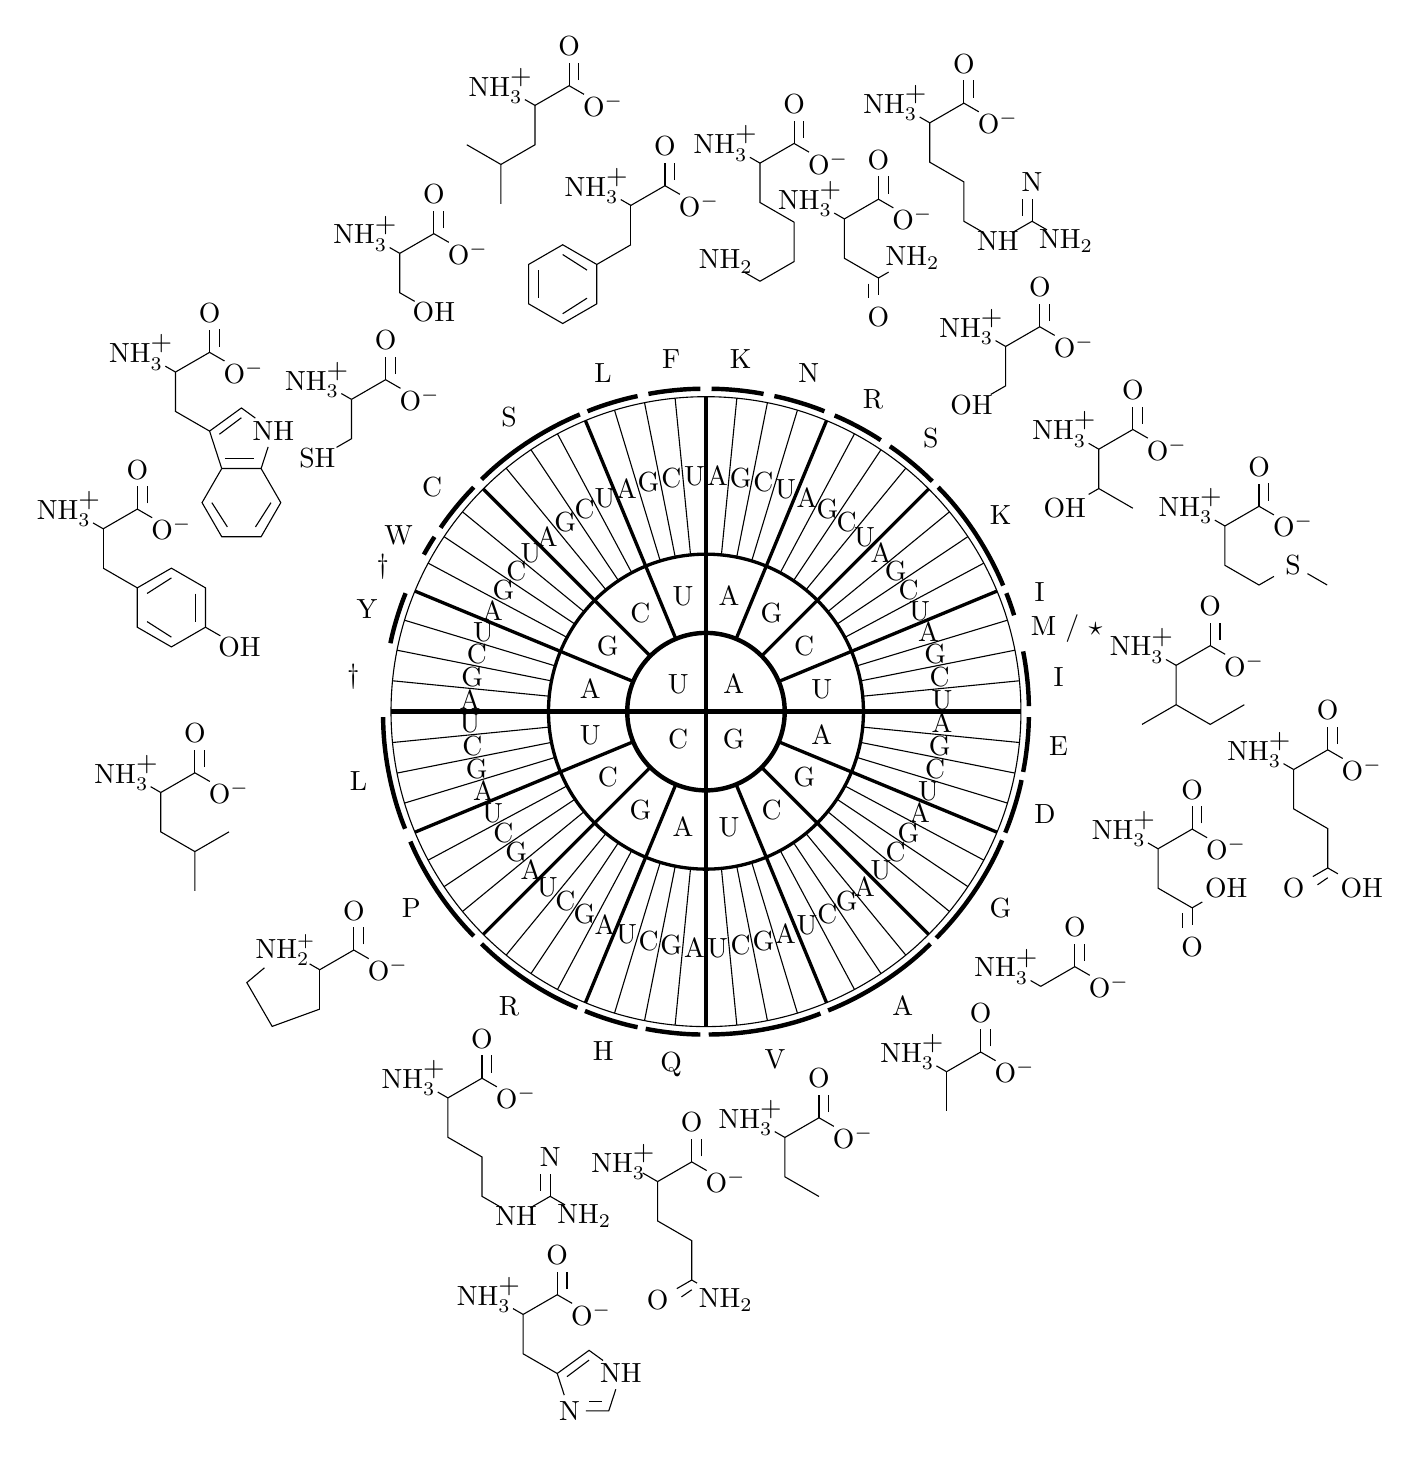
\begin{tikzpicture}
\begin{scope}
\draw [ultra thick] circle(1cm);
\draw [ultra thick] (0:4)--(180:4) (90:4)--(270:4);
\foreach \a/\l in {45/A,135/G,225/C,315/U}{
	\node at (90-\a:0.5cm) {\l};
}
\draw [very thick] circle(2cm);% (0:4)--(180:4) (90:4)--(270:4);
%\foreach \A in {0,90,180,270}{
\foreach \A in {90,0,270,180}{
\foreach \a/\l in {22.5/A,45/G,67.5/C,90/U}{
	\draw [very thick] (\A+\a:1) -- (\A+\a:4);
	\node at (\A-\a+11.25:1.5) {\l};
}
}
\draw circle(4cm) (0:4)--(180:4) (90:4)--(270:4);
\foreach \A in {90,180,270,0}{
\foreach \a in {0,22.5,45,67.5}{
\foreach \i/\l in {5.625/A,11.25/G,16.875/C,22.5/U}{
	\draw (\A+\a+\i:2) -- (\A+\a+\i:4);
	\node at (\A-\a-\i+2.8125:3) {\l};
}
}
}
\end{scope}
\begin{scope}[scale=0.5,relative=false]%K
\draw[ultra thick,shorten >=2pt,shorten <=2pt] (90:8.2) arc(90:90-2*5.625:8.2);
\path (90-1*5.625:14) node (zero) {};
\draw[shorten >=8pt] (zero.center) -- ++(30:1) node (CO) {}  -- +(330:1) node {O$^-$};
%\draw[double,shorten >=6pt] (30:1)  -- +(90:1) node {O};
\draw[shorten >=6pt] (CO.center)  -- +(90:1) node (Od) {O};
\draw[shorten >=8pt] (CO.30)  -- +(90:1);
\draw[shorten >=10pt] (zero.center) -- ++(150:1) node {NH$_3^{\mbox{+}}$};
\draw[shorten >=8pt] (zero.center) -- ++(270:1) node(Cb){} -- ++(330:1) node (Cc) {}  -- ++(270:1) node (Cd) {} -- ++(210:1) node (Ce) {}  -- ++(150:1) node (Cf) {NH$_2$};
\end{scope}
\begin{scope}[scale=0.5,relative=false]%N
\draw[ultra thick,shorten >=2pt,shorten <=2pt] (90-2*5.625:8.2) arc(90-2*5.625:90-4*5.625:8.2);
\path (90-3.5*3.625-3:13) node (zero) {};
\draw[shorten >=8pt] (zero.center) -- ++(30:1) node (CO) {}  -- +(330:1) node {O$^-$};
%\draw[double,shorten >=6pt] (30:1)  -- +(90:1) node {O};
\draw[shorten >=6pt] (CO.center)  -- +(90:1) node (Od) {O};
\draw[shorten >=8pt] (CO.30)  -- +(90:1);
\draw[shorten >=10pt] (zero.center) -- ++(150:1) node {NH$_3^{\mbox{+}}$};
\draw[shorten >=10pt] (zero.center) -- ++(270:1) node(Cb){} -- ++(330:1) node (Cc) {}  -- +(30:1) node (Cd) {NH$_2$};
\draw[shorten >=8pt] (Cc.center) -- +(270:1) node (O) {};
\draw[shorten >=5pt] (Cc.210) -- (O.150);
\path (O.center) node {O};
\end{scope}
\begin{scope}[scale=0.5,relative=false]%R
\draw[ultra thick,shorten >=2pt,shorten <=2pt] (90-22.5:8.2) arc(90-22.5:90-33.75:8.2);
\path (90-3.7*5.625:16) node (zero) {};
\draw[shorten >=8pt] (zero.center) -- ++(30:1) node (CO) {}  -- +(330:1) node {O$^-$};
%\draw[double,shorten >=6pt] (30:1)  -- +(90:1) node {O};
\draw[shorten >=6pt] (CO.center)  -- +(90:1) node (Od) {O};
\draw[shorten >=8pt] (CO.30)  -- +(90:1);
\draw[shorten >=10pt] (zero.center) -- ++(150:1) node {NH$_3^{\mbox{+}}$};
\draw[shorten >=6pt] (zero.center) -- ++(270:1) node(Cb){} -- ++(330:1) node (Cc) {} -- ++(270:1) node (Cd) {} -- ++(330:1) node (NH1) {NH};
\draw[shorten <=6pt,shorten >=8pt] (NH1.center)-- ++(30:1) node (Ce) {} -- ++(330:1) node {NH$_2$};
\draw[shorten >=6pt] (Ce.center) -- ++(90:1) node (N2) {};
\draw[shorten >=4pt] (Ce.150) -- (N2.210);
\path (N2) node {N};
\end{scope}
\begin{scope}[scale=0.5,relative=false]%S
\draw[ultra thick,shorten >=1pt,shorten <=2pt] (90-22.5-2*5.625:8.2) arc(90-33.75:90-33.75-11.25:8.2);
\path (90-7*5.625:12) node (zero) {};
\draw[shorten >=8pt] (zero.center) -- ++(30:1) node (CO) {}  -- +(330:1) node {O$^-$};
%\draw[double,shorten >=6pt] (30:1)  -- +(90:1) node {O};
\draw[shorten >=6pt] (CO.center)  -- +(90:1) node (Od) {O};
\draw[shorten >=8pt] (CO.30)  -- +(90:1);
\draw[shorten >=10pt] (zero.center) -- ++(150:1) node {NH$_3^{\mbox{+}}$};
\draw[shorten >=8pt] (zero.center) -- ++(270:1) node(Cb){} -- ++(210:1) node (Cc) {OH};
\end{scope}
\begin{scope}[scale=0.5,relative=false]%T
\draw[ultra thick,shorten >=1pt,shorten <=2pt] (90-45:8.2) arc(90-45:90-67.5:8.2);
\path (90-45-11.25:12) node (zero) {};
\draw[shorten >=8pt] (zero.center) -- ++(30:1) node (CO) {}  -- +(330:1) node {O$^-$};
%\draw[double,shorten >=6pt] (30:1)  -- +(90:1) node {O};
\draw[shorten >=6pt] (CO.center)  -- +(90:1) node (Od) {O};
\draw[shorten >=8pt] (CO.30)  -- +(90:1);
\draw[shorten >=10pt] (zero.center) -- ++(150:1) node {NH$_3^{\mbox{+}}$};
\draw[shorten >=10pt] (zero.center) -- ++(270:1) node(Cb){} -- ++(330:1) node (Cc) {} (Cb.center) -- +(210:1) node {OH};
\end{scope}
\begin{scope}[scale=0.5,relative=false]%M
\draw[ultra thick,shorten >=1pt,shorten <=2pt] (90-67.5:8.2) arc(90-67.5:90-67.5-5.625:8.2);
\path (90-67.5-0.5*5.625:14) node (zero) {};
\draw[shorten >=8pt] (zero.center) -- ++(30:1) node (CO) {}  -- +(330:1) node {O$^-$};
%\draw[double,shorten >=6pt] (30:1)  -- +(90:1) node {O};
\draw[shorten >=6pt] (CO.center)  -- +(90:1) node (Od) {O};
\draw[shorten >=8pt] (CO.30)  -- +(90:1);
\draw[shorten >=10pt] (zero.center) -- ++(150:1) node {NH$_3^{\mbox{+}}$};
\draw[shorten >=8pt] (zero.center) -- ++(270:1) node(Cb){} -- ++(330:1) node (Cc) {}  -- ++(30:1) node (Cd) {S};
\draw[shorten <=6pt] (Cd.center) -- +(330:1);
\end{scope}
\begin{scope}[scale=0.5,relative=false]%I
\draw[ultra thick,shorten >=1pt,shorten <=2pt] (0:8.2) arc(0:11.25:8.2);
\path (5.625:12) node (zero) {};
\draw[shorten >=8pt] (zero.center) -- ++(30:1) node (CO) {}  -- +(330:1) node {O$^-$};
%\draw[double,shorten >=6pt] (30:1)  -- +(90:1) node {O};
\draw[shorten >=6pt] (CO.center)  -- +(90:1) node (Od) {O};
\draw[shorten >=8pt] (CO.30)  -- +(90:1);
\draw[shorten >=10pt] (zero.center) -- ++(150:1) node {NH$_3^{\mbox{+}}$};
\draw (zero.center) -- ++(270:1) node(Cb){} -- ++(330:1) node (Cc) {}  -- +(30:1) node (Cd) {} (Cb.center) -- +(210:1) node (Ce) {};
\end{scope}
\begin{scope}[scale=0.5,relative=false]%E
\draw[ultra thick,shorten >=1pt,shorten <=2pt] (0:8.2) arc(0:-11.25:8.2);
\path (-5.625:15) node (zero) {};
\draw[shorten >=8pt] (zero.center) -- ++(30:1) node (CO) {}  -- +(330:1) node {O$^-$};
%\draw[double,shorten >=6pt] (30:1)  -- +(90:1) node {O};
\draw[shorten >=6pt] (CO.center)  -- +(90:1) node (Od) {O};
\draw[shorten >=8pt] (CO.30)  -- +(90:1);
\draw[shorten >=10pt] (zero.center) -- ++(150:1) node {NH$_3^{\mbox{+}}$};
\draw[shorten >=10pt] (zero.center) -- ++(270:1) node(Cb){} -- ++(330:1) node (Cc) {} -- ++(270:1) node (Cd) {} -- ++(330:1) node (NH) {OH};
\draw[shorten >=8pt] (Cd.center) -- +(210:1) node (O) {};
\draw[shorten >=8pt] (Cd.270) -- (O.300);
\path (O.center) node {O};
\end{scope}
\begin{scope}[scale=0.5,relative=false]%D
\draw[ultra thick,shorten >=1pt,shorten <=2pt] (-11.25:8.2) arc(-11.25:-22.5:8.2);
\path (-11.25-5.625:12) node (zero) {};
\draw[shorten >=8pt] (zero.center) -- ++(30:1) node (CO) {}  -- +(330:1) node {O$^-$};
%\draw[double,shorten >=6pt] (30:1)  -- +(90:1) node {O};
\draw[shorten >=6pt] (CO.center)  -- +(90:1) node (Od) {O};
\draw[shorten >=8pt] (CO.30)  -- +(90:1);
\draw[shorten >=10pt] (zero.center) -- ++(150:1) node {NH$_3^{\mbox{+}}$};
\draw[shorten >=10pt] (zero.center) -- ++(270:1) node(Cb){} -- ++(330:1) node (Cc) {}  -- +(30:1) node (Cd) {OH};
\draw[shorten >=8pt] (Cc.center) -- +(270:1) node (O) {};
\draw[shorten >=5pt] (Cc.210) -- (O.150);
\path (O.center) node {O};
\end{scope}
\begin{scope}[scale=0.5,relative=false]%G
\draw[ultra thick,shorten >=1pt,shorten <=2pt] (-22.5:8.2) arc(-22.5:-45:8.2);
\path (-33.75-1*5.625:11) node (zero) {};
\draw[shorten >=8pt] (zero.center) -- ++(30:1) node (CO) {}  -- +(330:1) node {O$^-$};
%\draw[double,shorten >=6pt] (30:1)  -- +(90:1) node {O};
\draw[shorten >=6pt] (CO.center)  -- +(90:1) node (Od) {O};
\draw[shorten >=8pt] (CO.30)  -- +(90:1);
\draw[shorten >=10pt] (zero.center) -- ++(150:1) node {NH$_3^{\mbox{+}}$};
\end{scope}
\begin{scope}[scale=0.5,relative=false]%A
\draw[ultra thick,shorten >=1pt,shorten <=2pt] (-45:8.2) arc(-45:-68.25:8.2);
\path (-45-11.25:11) node (zero) {};
\draw[shorten >=8pt] (zero.center) -- ++(30:1) node (CO) {}  -- +(330:1) node {O$^-$};
%\draw[double,shorten >=6pt] (30:1)  -- +(90:1) node {O};
\draw[shorten >=6pt] (CO.center)  -- +(90:1) node (Od) {O};
\draw[shorten >=8pt] (CO.30)  -- +(90:1);
\draw[shorten >=10pt] (zero.center) -- ++(150:1) node {NH$_3^{\mbox{+}}$};
\draw (zero.center) -- ++(270:1) node(Cb){};
\end{scope}
\begin{scope}[scale=0.5,relative=false]%V
\draw[ultra thick,shorten >=1pt,shorten <=2pt] (-68.25:8.2) arc(-68.25:-90:8.2);
\path (-68.25-11.25:11) node (zero) {};
\draw[shorten >=8pt] (zero.center) -- ++(30:1) node (CO) {}  -- +(330:1) node {O$^-$};
%\draw[double,shorten >=6pt] (30:1)  -- +(90:1) node {O};
\draw[shorten >=6pt] (CO.center)  -- +(90:1) node (Od) {O};
\draw[shorten >=8pt] (CO.30)  -- +(90:1);
\draw[shorten >=10pt] (zero.center) -- ++(150:1) node {NH$_3^{\mbox{+}}$};
\draw (zero.center) -- ++(270:1) node(Cb){} -- ++(330:1) node (Cc) {};
\end{scope}
\begin{scope}[scale=0.5,relative=false]%Q
\draw[ultra thick,shorten >=1pt,shorten <=2pt] (-90:8.2) arc(-90:-101.25:8.2);
\path (-90.25-5.625:12) node (zero) {};
\draw[shorten >=8pt] (zero.center) -- ++(30:1) node (CO) {}  -- +(330:1) node {O$^-$};
%\draw[double,shorten >=6pt] (30:1)  -- +(90:1) node {O};
\draw[shorten >=6pt] (CO.center)  -- +(90:1) node (Od) {O};
\draw[shorten >=8pt] (CO.30)  -- +(90:1);
\draw[shorten >=8pt] (zero.center) -- ++(150:1) node {NH$_3^{\mbox{+}}$};
\draw[shorten >=12pt] (zero.center) -- ++(270:1) node(Cb){} -- ++(330:1) node (Cc) {} -- ++(270:1) node (Cd) {} -- ++(330:1) node (NH) {NH$_2$};
\draw[shorten >=8pt] (Cd.center) -- +(210:1) node (O) {};
\draw[shorten >=8pt] (Cd.270) -- (O.300);
\path (O.center) node {O};
\end{scope}
\begin{scope}[scale=0.5,relative=false]%H
\draw[ultra thick,shorten >=1pt,shorten <=2pt] (-101.25:8.2) arc(-101.25:-101.25-11.25:8.2);
\path (-101.25-5.625:16) node (zero) {};
\draw[shorten >=8pt] (zero.center) -- ++(30:1) node (CO) {}  -- +(330:1) node {O$^-$};
\draw[shorten >=6pt] (CO.center)  -- +(90:1) node (Od) {O};
\draw[shorten >=8pt] (CO.30)  -- +(90:1);
\draw[shorten >=10pt] (zero.center) -- ++(150:1) node {NH$_3^{\mbox{+}}$};
\draw (zero.center) -- ++(270:1) node(Cb){}  -- ++(330:1) node(Cc){};
\draw[shorten >=8pt] (Cc.center) -- ++(108-1*72:1) node (Cd) {}
	 -- ++(108-2*72:1) node (Ce) {NH};
\draw[shorten <=6pt,shorten >=6pt] (Ce.center) -- ++(108-3*72:1) node (Cf) {}
	 -- ++(108-4*72:1) node (Cg) {};
\draw[shorten <=6pt] (Cg.center) -- (Cc.center);
\draw (Cc.198+2*72) -- (Cd.198+1*72);
\draw[shorten <=6pt] (Cg.72) -- (Cf.198+4*72);
\draw (Cg.center) node {N};
\end{scope}
\begin{scope}[scale=0.5,relative=false]%R
\draw[ultra thick,shorten >=2pt,shorten <=2pt] (-90-22.5:8.2) arc(-90-22.5:-90-45:8.2);
\path (-90-6*5.625:11.8) node (zero) {};
\draw[shorten >=8pt] (zero.center) -- ++(30:1) node (CO) {}  -- +(330:1) node {O$^-$};
%\draw[double,shorten >=6pt] (30:1)  -- +(90:1) node {O};
\draw[shorten >=6pt] (CO.center)  -- +(90:1) node (Od) {O};
\draw[shorten >=8pt] (CO.30)  -- +(90:1);
\draw[shorten >=10pt] (zero.center) -- ++(150:1) node {NH$_3^{\mbox{+}}$};
\draw[shorten >=6pt] (zero.center) -- ++(270:1) node(Cb){} -- ++(330:1) node (Cc) {} -- ++(270:1) node (Cd) {} -- ++(330:1) node (NH1) {NH};
\draw[shorten <=6pt,shorten >=8pt] (NH1.center)-- ++(30:1) node (Ce) {} -- ++(330:1) node {NH$_2$};
\draw[shorten >=6pt] (Ce.center) -- ++(90:1) node (N2) {};
\draw[shorten >=4pt] (Ce.150) -- (N2.210);
\path (N2) node {N};
\end{scope}
\begin{scope}[scale=0.5,relative=false]%P
\draw[ultra thick,shorten >=2pt,shorten <=2pt] (-90-45:8.2) arc(-90-45:-90-45-22.25:8.2);
\path (-90-10*5.625:11.8) node (zero) {};
\draw[shorten >=8pt] (zero.center) -- ++(30:1) node (CO) {}  -- +(330:1) node {O$^-$};
%\draw[double,shorten >=6pt] (30:1)  -- +(90:1) node {O};
\draw[shorten >=6pt] (CO.center)  -- +(90:1) node (Od) {O};
\draw[shorten >=8pt] (CO.30)  -- +(90:1);
\draw[shorten >=10pt] (zero.center) -- ++(150:1) node (nh) {NH$_2^+$};
\draw (zero.center) -- ++(270:1) node(Cb){};
\path (Cb.center) -- +(150:1) node (x) {};
\path (x.center)  +(170:1) node (Cd) {};
\path (x.center)  +(250:1) node (Cc) {};
\draw[shorten >=10pt] (Cb.center) -- (Cc.center) -- (Cd.center) -- (nh.center);
\end{scope}
\begin{scope}[scale=0.5,relative=false]%L
\draw[ultra thick,shorten >=2pt,shorten <=2pt] (180:8.2) arc(180:180+22.25:8.2);
\path (-90-14.5*5.625:14) node (zero) {};
\draw[shorten >=8pt] (zero.center) -- ++(30:1) node (CO) {}  -- +(330:1) node {O$^-$};
%\draw[double,shorten >=6pt] (30:1)  -- +(90:1) node {O};
\draw[shorten >=6pt] (CO.center)  -- +(90:1) node (Od) {O};
\draw[shorten >=8pt] (CO.30)  -- +(90:1);
\draw[shorten >=10pt] (zero.center) -- ++(150:1) node {NH$_3^{\mbox{+}}$};
\draw (zero.center) -- ++(270:1) node(Cb){} -- ++(330:1) node (Cc) {}  -- +(30:1) node (Cd) {} (Cc.center) -- +(270:1) node (Ce) {};
\end{scope}
\begin{scope}[scale=0.5,relative=false]%Y
\draw[ultra thick,shorten >=2pt,shorten <=2pt] (180-11.25:8.2) arc(180-11.25:180-22.5:8.2);
\path (180-3*5.625:16) node (zero) {};
\draw[shorten >=8pt] (zero.center) -- ++(30:1) node (CO) {}  -- +(330:1) node {O$^-$};
%\draw[double,shorten >=6pt] (30:1)  -- +(90:1) node {O};
\draw[shorten >=6pt] (CO.center)  -- +(90:1) node (Od) {O};
\draw[shorten >=8pt] (CO.30)  -- +(90:1);
\draw[shorten >=10pt] (zero.center) -- ++(150:1) node {NH$_3^{\mbox{+}}$};
\draw (zero.center) -- ++(270:1) node(Cb){};
\draw (Cb.center) -- ++(330:1) node (Cc) {} -- ++(30:1) node (Cd) {} -- ++(330:1) node (Ce) {} -- ++(270:1) node (Cf) {}
	-- ++(210:1) node (Cg) {} -- ++(150:1) node (Ch) {} -- ++(90:1);
\draw (Cc.330) -- (Cd.270);
\draw (Ce.210) -- (Cf.150);
\draw (Cg.90) -- (Ch.30);
\draw[shorten >=8pt] (Cf.center) -- +(330:1) node (OH) {OH};
\end{scope}
\begin{scope}[scale=0.5,relative=false]%W
\draw[ultra thick,shorten >=2pt,shorten <=2pt] (180-22.5-5.625:8.2) arc(180-22.5-5.625:180-22.5-11.25:8.2);
\path (180-22.5-1.8*5.625:16) node (zero) {};
\draw[shorten >=8pt] (zero.center) -- ++(30:1) node (CO) {}  -- +(330:1) node {O$^-$};
%\draw[double,shorten >=6pt] (30:1)  -- +(90:1) node {O};
\draw[shorten >=6pt] (CO.center)  -- +(90:1) node (Od) {O};
\draw[shorten >=8pt] (CO.30)  -- +(90:1);
\draw[shorten >=10pt] (zero.center) -- ++(150:1) node {NH$_3^{\mbox{+}}$};
\draw (zero.center) -- ++(270:1) node(Cb){}  -- ++(330:1) node(Cc){};
\draw[shorten >=8pt] (Cc.center) -- ++(108-1*72:1) node (Cd) {}
	 -- ++(108-2*72:1) node (Ce) {NH};
\draw[shorten <=6pt] (Ce.center) -- ++(108-3*72:1) node (Cf) {}
	 -- ++(108-4*72:1) node (Cg) {};
\draw[shorten <=0pt] (Cg.center) -- (Cc.center);
\draw (Cc.198+2*72) -- (Cd.198+1*72);
\draw[shorten <=0pt] (Cg.72) -- (Cf.198+4*72);
\draw (Cg.center) -- ++(240:1) node (Ch) {} -- ++(300:1) node (Ci) {} -- ++(0:1) node (Cj) {}
	 -- ++(60:1) node (Ck) {} -- ++(120:1) node (Cl) {};
\draw (Ch.0) -- (Ci.60);
\draw (Cj.120) -- (Ck.180);
\end{scope}
\begin{scope}[scale=0.5,relative=false]%C
\draw[ultra thick,shorten >=2pt,shorten <=2pt] (180-45+11.25:8.2) arc(180-45+11.25:180-45:8.2);
\path (180-45+11.25-1*7.625:12) node (zero) {};
\draw[shorten >=8pt] (zero.center) -- ++(30:1) node (CO) {}  -- +(330:1) node {O$^-$};
%\draw[double,shorten >=6pt] (30:1)  -- +(90:1) node {O};
\draw[shorten >=6pt] (CO.center)  -- +(90:1) node (Od) {O};
\draw[shorten >=8pt] (CO.30)  -- +(90:1);
\draw[shorten >=10pt] (zero.center) -- ++(150:1) node {NH$_3^{\mbox{+}}$};
\draw[shorten >=8pt] (zero.center) -- ++(270:1) node(Cb){} -- ++(210:1) node (Cc) {SH};
\end{scope}
\begin{scope}[scale=0.5,relative=false]%S
\draw[ultra thick,shorten >=1pt,shorten <=2pt] (90+45:8.2) arc(90+45:90+45-22.5:8.2);
\path (90+45-11.25+0*5.625:14) node (zero) {};
\draw[shorten >=8pt] (zero.center) -- ++(30:1) node (CO) {}  -- +(330:1) node {O$^-$};
%\draw[double,shorten >=6pt] (30:1)  -- +(90:1) node {O};
\draw[shorten >=6pt] (CO.center)  -- +(90:1) node (Od) {O};
\draw[shorten >=8pt] (CO.30)  -- +(90:1);
\draw[shorten >=10pt] (zero.center) -- ++(150:1) node {NH$_3^{\mbox{+}}$};
\draw[shorten >=8pt] (zero.center) -- ++(270:1) node(Cb){} -- ++(330:1) node (Cc) {OH};
\end{scope}
\begin{scope}[scale=0.5,relative=false]%L
\draw[ultra thick,shorten >=2pt,shorten <=2pt] (90+22.5:8.2) arc(90+22.5:90+11.25:8.2);
\path (90+22.5-1.2*5.625:16) node (zero) {};
\draw[shorten >=8pt] (zero.center) -- ++(30:1) node (CO) {}  -- +(330:1) node {O$^-$};
%\draw[double,shorten >=6pt] (30:1)  -- +(90:1) node {O};
\draw[shorten >=6pt] (CO.center)  -- +(90:1) node (Od) {O};
\draw[shorten >=8pt] (CO.30)  -- +(90:1);
\draw[shorten >=10pt] (zero.center) -- ++(150:1) node {NH$_3^{\mbox{+}}$};
\draw (zero.center) -- ++(270:1) node(Cb){} -- ++(210:1) node (Cc) {}  -- +(150:1) node (Cd) {} (Cc.center) -- +(270:1) node (Ce) {};
\end{scope}
\begin{scope}[scale=0.5,relative=false]%F
\draw[ultra thick,shorten >=2pt,shorten <=2pt] (90+11.25:8.2) arc(90+11.25:90:8.2);
\path (90+1.5*5.625:13) node (zero) {};
\draw[shorten >=8pt] (zero.center) -- ++(30:1) node (CO) {}  -- +(330:1) node {O$^-$};
%\draw[double,shorten >=6pt] (30:1)  -- +(90:1) node {O};
\draw[shorten >=6pt] (CO.center)  -- +(90:1) node (Od) {O};
\draw[shorten >=8pt] (CO.30)  -- +(90:1);
\draw[shorten >=10pt] (zero.center) -- ++(150:1) node {NH$_3^{\mbox{+}}$};
\draw (zero.center) -- ++(270:1) node(Cb){};
\draw (Cb.center) -- ++(210:1) node (Cc) {} -- ++(150:1) node (Cd) {}
	-- ++(210:1) node (Ce) {} -- ++(270:1) node (Cf) {}
	-- ++(330:1) node (Cg) {} -- ++(30:1) node (Ch) {} -- ++(90:1);
\draw (Cc.210) -- (Cd.270);
\draw (Ce.330) -- (Cf.30);
\draw (Cg.90) -- (Ch.150);
\end{scope}
\node at (90-1*5.625:4.5) {K};
\node at (90-3*5.625:4.5) {N};
\node at (90-5*5.625:4.5) {R};
\node at (90-7*5.625:4.5) {S};
\node at (90-10*5.625:4.5) {K};
\node at (90-12.5*5.625:4.5) {I};
\node at (90-13.7*5.625:4.7) {M / $\star$};
\node at (90-15*5.625:4.5) {I};
\node at (90-17*5.625:4.5) {E};
\node at (90-19*5.625:4.5) {D};
\node at (90-22*5.625:4.5) {G};
\node at (90-26*5.625:4.5) {A};
\node at (90-30*5.625:4.5) {V};
\node at (90-33*5.625:4.5) {Q};
\node at (90-35*5.625:4.5) {H};
\node at (90-38*5.625:4.5) {R};
\node at (90-42*5.625:4.5) {P};
\node at (90-46*5.625:4.5) {L};
\node at (90-49*5.625:4.5) {$\dagger$};
\node at (90-51*5.625:4.5) {Y};
\node at (90-52.3*5.625:4.5) {$\dagger$};
\node at (90-53.3*5.625:4.5) {W};
\node at (90-55*5.625:4.5) {C};
\node at (90-58*5.625:4.5) {S};
\node at (90-61*5.625:4.5) {L};
\node at (90-63*5.625:4.5) {F};
\end{tikzpicture}
\end{center}
\end{document}
